\documentclass[tikz,border=10pt]{standalone}
\usepackage{amsmath,amssymb}
\usepackage{tikz}
\usetikzlibrary{shapes.geometric,arrows.meta,positioning,calc,fit,backgrounds}

\begin{document}
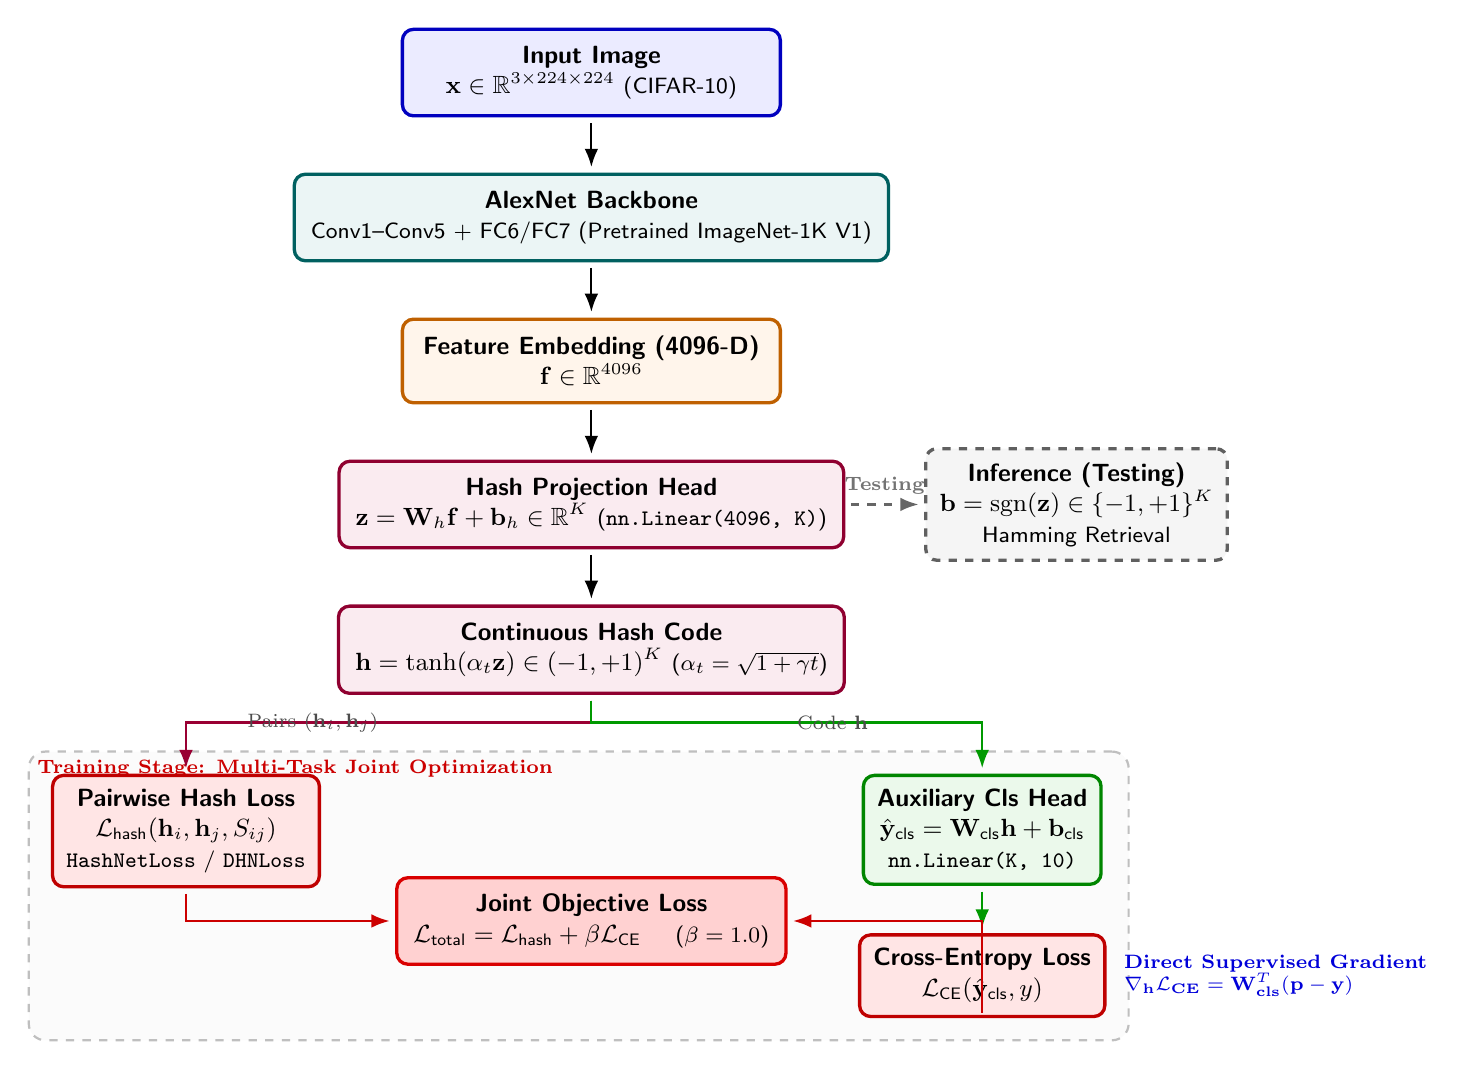
\begin{tikzpicture}[
    >=Latex,
    font=\sffamily\small,
    % Standardized, publication-ready block styles
    block/.style={
        rectangle, draw=#1!75!black, fill=#1!8, very thick,
        rounded corners=4pt, align=center,
        inner sep=6pt, minimum height=0.95cm, minimum width=4.8cm
    },
    block/.default=blue,
    branchblock/.style={
        rectangle, draw=#1!75!black, fill=#1!8, very thick,
        rounded corners=4pt, align=center,
        inner sep=5pt, minimum height=0.95cm, minimum width=3.0cm
    },
    branchblock/.default=blue,
    lossblock/.style={
        rectangle, draw=red!75!black, fill=red!10, very thick,
        rounded corners=4pt, align=center,
        inner sep=5pt, minimum height=0.95cm, minimum width=3.0cm
    },
    inferblock/.style={
        rectangle, draw=gray!75!black, fill=gray!8, dashed, very thick,
        rounded corners=4pt, align=center,
        inner sep=5pt, minimum height=0.95cm, minimum width=2.6cm
    },
    totallossblock/.style={
        rectangle, draw=red!85!black, fill=red!18, very thick,
        rounded corners=4pt, align=center,
        inner sep=6pt, minimum height=1.0cm, minimum width=4.8cm
    },
    stagebox/.style={
        draw=black!25, fill=black!1.5, rounded corners=6pt,
        inner sep=8pt, dashed, thick
    },
    conn/.style={->, thick, shorten >=2pt, shorten <=2pt},
    annot/.style={font=\scriptsize, text=black!70}
]

    % =========================================================================
    % MAIN VERTICAL BACKBONE: TOP TO BOTTOM
    % =========================================================================
    % 1. Input Image
    \node[block=blue] (input) {
        \textbf{Input Image}\\
        $\mathbf{x} \in \mathbb{R}^{3 \times 224 \times 224}$ \footnotesize (CIFAR-10)
    };

    % 2. AlexNet Backbone
    \node[block=teal, below=0.7cm of input] (backbone) {
        \textbf{AlexNet Backbone}\\
        \footnotesize Conv1--Conv5 + FC6/FC7 (Pretrained ImageNet-1K V1)
    };

    % 3. Feature Embedding (4096-D)
    \node[block=orange, below=0.7cm of backbone] (feat) {
        \textbf{Feature Embedding (4096-D)}\\
        $\mathbf{f} \in \mathbb{R}^{4096}$
    };

    % 4. Hash Projection
    \node[block=purple, below=0.7cm of feat] (hashproj) {
        \textbf{Hash Projection Head}\\
        $\mathbf{z} = \mathbf{W}_h \mathbf{f} + \mathbf{b}_h \in \mathbb{R}^K$ \footnotesize (\texttt{nn.Linear(4096, K)})
    };

    % 5. Continuous Hash Code
    \node[block=purple, below=0.7cm of hashproj] (tanh) {
        \textbf{Continuous Hash Code}\\
        $\mathbf{h} = \tanh(\alpha_t \mathbf{z}) \in (-1, +1)^K$ \footnotesize ($\alpha_t = \sqrt{1 + \gamma t}$)
    };

    % Main vertical connectors
    \draw[conn] (input) -- (backbone);
    \draw[conn] (backbone) -- (feat);
    \draw[conn] (feat) -- (hashproj);
    \draw[conn] (hashproj) -- (tanh);

    % =========================================================================
    % INFERENCE BRANCH (TESTING STAGE - SEPARATED TO THE RIGHT)
    % =========================================================================
    \node[inferblock, right=1.0cm of hashproj] (infer) {
        \textbf{Inference (Testing)}\\
        $\mathbf{b} = \mathrm{sgn}(\mathbf{z}) \in \{-1, +1\}^K$\\
        \footnotesize Hamming Retrieval
    };
    \draw[conn, dashed, gray!80!black] (hashproj.east) -- (infer.west)
        node[midway, above, font=\scriptsize\bfseries, text=gray!90!black] {Testing};

    % =========================================================================
    % MULTI-TASK DUAL BRANCHES (TRAINING STAGE)
    % =========================================================================
    % Branch 1 (Left): Pairwise Hash Loss
    \node[lossblock, below left=1.0cm and 0.2cm of tanh] (hashloss) {
        \textbf{Pairwise Hash Loss}\\
        $\mathcal{L}_{\text{hash}}(\mathbf{h}_i, \mathbf{h}_j, S_{ij})$\\
        \footnotesize \texttt{HashNetLoss} / \texttt{DHNLoss}
    };

    % Branch 2 (Right): Auxiliary Classification Head
    \node[branchblock=green!70!black, below right=1.0cm and 0.2cm of tanh] (clshead) {
        \textbf{Auxiliary Cls Head}\\
        $\hat{\mathbf{y}}_{\text{cls}} = \mathbf{W}_{\text{cls}} \mathbf{h} + \mathbf{b}_{\text{cls}}$\\
        \footnotesize \texttt{nn.Linear(K, 10)}
    };

    % Cross-Entropy Loss directly beneath Auxiliary Cls Head
    \node[lossblock, below=0.6cm of clshead] (clsloss) {
        \textbf{Cross-Entropy Loss}\\
        $\mathcal{L}_{\text{CE}}(\hat{\mathbf{y}}_{\text{cls}}, y)$
    };

    % Split connectors from continuous code
    \draw[conn, purple!80!black] (tanh.south) -- ++(0, -0.35) -| (hashloss.north)
        node[pos=0.25, left, annot] {Pairs $(\mathbf{h}_i, \mathbf{h}_j)$};
    \draw[conn, green!60!black] (tanh.south) -- ++(0, -0.35) -| (clshead.north)
        node[pos=0.25, right, annot] {Code $\mathbf{h}$};

    \draw[conn, green!60!black] (clshead) -- (clsloss);

    % =========================================================================
    % JOINT OBJECTIVE LOSS (CONVERGENCE AT BOTTOM)
    % =========================================================================
    \node[totallossblock, below=2.3cm of tanh] (totalloss) {
        \textbf{Joint Objective Loss}\\
        $\mathcal{L}_{\text{total}} = \mathcal{L}_{\text{hash}} + \beta \mathcal{L}_{\text{CE}}$ \quad \footnotesize ($\beta = 1.0$)
    };

    % Merge connectors
    \draw[conn, red!80!black] (hashloss.south) |- (totalloss.west);
    \draw[conn, red!80!black] (clsloss.south) |- (totalloss.east);

    % Direct gradient indication (clean, professional side label)
    \path (clsloss.east) -- ++(0.1, 0) node[right, font=\scriptsize\bfseries, text=blue!85!black, align=left] {
        Direct Supervised Gradient\\
        $\nabla_{\mathbf{h}} \mathcal{L}_{\text{CE}} = \mathbf{W}_{\text{cls}}^T (\mathbf{p} - \mathbf{y})$
    };

    % Background group for Training vs Testing clarity
    \begin{scope}[on background layer]
        \node[stagebox, fit=(hashloss) (clshead) (clsloss) (totalloss),
              label={[anchor=north west, font=\scriptsize\bfseries, text=red!80!black]north west:Training Stage: Multi-Task Joint Optimization}] {};
    \end{scope}

\end{tikzpicture}
\end{document}
